\input{BASE-HEAD}
\newcommand{\laClass}       {CS 211}
\newcommand{\laSemester}    {Spring 2018}
\newcommand{\laChapter}     {7.3}
\newcommand{\laType}        {Exercise}
\newcommand{\laPoints}      {5}
\newcommand{\laTitle}       {Isomorphism and Planarity}
\newcommand{\laDate}        {}
\setcounter{chapter}{7}
\setcounter{section}{3}
\addtocounter{section}{-1}
\newcounter{question}

\toggletrue{answerkey}


\title{}
\author{Rachel Singh}
\date{\today}

\pagestyle{fancy}
\fancyhf{}

\lhead{\laClass}

\chead{\laSemester}

\rhead{\laChapter\ \laType\ \iftoggle{answerkey}{ KEY }{}}

\rfoot{\thepage\ of \pageref{LastPage}}

\lfoot{\scriptsize By Rachel Morris, last updated \today}

\renewcommand{\headrulewidth}{2pt}
\renewcommand{\footrulewidth}{1pt}

\begin{document}




\notonkey{

\footnotesize
~\\ 
\textbf{\laChapter\ \laType: } In-class exercises are meant to introduce you to a new topic
and provide some practice with the new topic. Work in a team of up to 4 people to complete this exercise.
You can work simultaneously on the problems, or work separate and then check your answers with each other.
You can take the exercise home, score will be based on the in-class quiz the following class period.
\textbf{Work out problems on your own paper} - this document just has examples and questions.

\hrulefill
\normalsize 

}{
\begin{center}
    \Large
    \textbf{Answer Key}
\end{center}
}



% KEY ------------------------------------ %

\begin{enumerate}
    \item   Multiple solutions, but here are some examples:
        \begin{itemize}
            \item[a.]
                \solution{
                    Example:
                    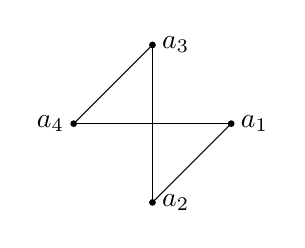
\begin{tikzpicture}
                        \filldraw (3,1) circle (1pt) node[right] {$a_{1}$};
                        \filldraw (2,0) circle (1pt) node[right] {$a_{2}$};
                        \filldraw (2,2) circle (1pt) node[right] {$a_{3}$};
                        \filldraw (1,1) circle (1pt) node[left] {$a_{4}$};

                        \draw (3,1) -- (2,0);
                        \draw (2,0) -- (2,2);
                        \draw (2,2) -- (1,1);
                        \draw (1,1) -- (3,1);
                    \end{tikzpicture}
                }{}
                
            \item[b.]
                \solution{
                    Example:
                    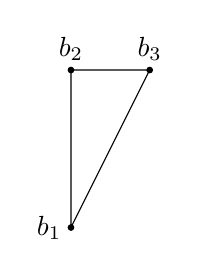
\begin{tikzpicture}
                        \filldraw (0,0) circle (1pt) node[left] {$b_{1}$};
                        \filldraw (0,2) circle (1pt) node[above] {$b_{2}$};
                        \filldraw (1,2) circle (1pt) node[above] {$b_{3}$};

                        \draw (0,0) -- (0,2) -- (1,2) -- (0,0);
                    \end{tikzpicture}
                }{}
        \end{itemize}
        
        \hrulefill
    \item
        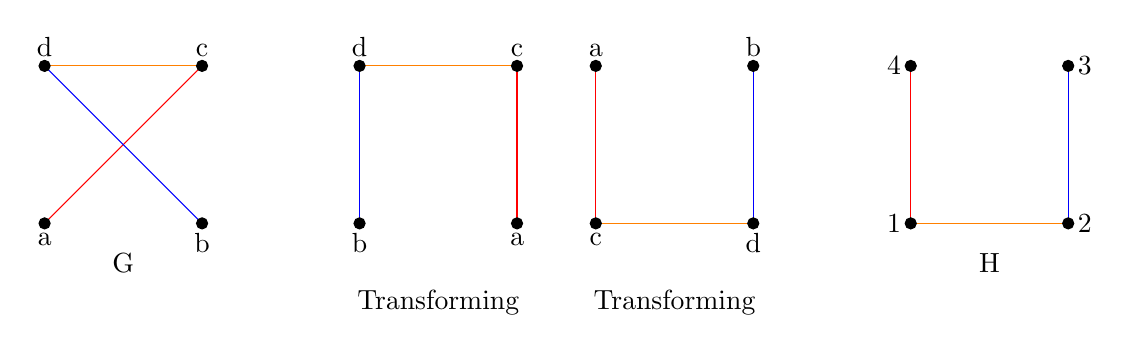
\begin{tikzpicture}
            \draw[red] (0,0) -- (2,2);
            \draw[orange] (2,2) -- (0,2);
            \draw[blue] (0,2) -- (2,0);
        
            \filldraw (0,0) circle (2pt) node[below] {a};
            \filldraw (2,0) circle (2pt) node[below] {b};
            \filldraw (2,2) circle (2pt) node[above] {c};
            \filldraw (0,2) circle (2pt) node[above] {d};

            \node at (1,-0.5) {G};

            \draw[red] (6,0) -- (6,2);
            \draw[orange] (6,2) -- (4,2);
            \draw[blue] (4,2) -- (4,0);
        
            \filldraw (6,0) circle (2pt) node[below] {a};
            \filldraw (4,0) circle (2pt) node[below] {b};
            \filldraw (6,2) circle (2pt) node[above] {c};
            \filldraw (4,2) circle (2pt) node[above] {d};

            \node at (5,-1) {Transforming};

            \draw[red] (7,2) -- (7,0);
            \draw[orange] (7,0) -- (9,0);
            \draw[blue] (9,0) -- (9,2);
        
            \filldraw (7,2) circle (2pt) node[above] {a};
            \filldraw (9,2) circle (2pt) node[above] {b};
            \filldraw (7,0) circle (2pt) node[below] {c};
            \filldraw (9,0) circle (2pt) node[below] {d};

            \node at (8,-1) {Transforming};

            \draw[blue]         (13,2) -- (13,0);
            \draw[orange]       (13,0) -- (11,0);
            \draw[red]          (11,0) -- (11,2);
        
            \filldraw   (13,2) circle (2pt) node[right] {3};
            \filldraw   (11,2) circle (2pt) node[left]   {4};
            \filldraw   (13,0) circle (2pt) node[right] {2};
            \filldraw   (11,0) circle (2pt) node[left]   {1};

            \node at (12, -0.5) {H};
        \end{tikzpicture}
        
        \item[a.]   Vertex Map:
            \begin{tabular}{c | c | c | c | c}
                G & a & b & c & d
                \\ \hline
                H
                &   \solution{ 4 }{}
                &   \solution{ 3 }{}
                &   \solution{ 1 }{}
                &   \solution{ 2 }{}
            \end{tabular}

        \normalsize
        \item[b.]   Edge Map:
            \begin{tabular}{c | c | c | c}
                G & \{a, c\} & \{c, d\} & \{d, b\}
                \\ \hline
                H
                &   \solution{ \{4,1\} }{}
                &   \solution{ \{1,2\} }{}
                &   \solution{ \{2,3\} }{}
            \end{tabular}

    \newpage
    \item   
        \begin{itemize}
            \item[a.]   Write out all edges for both graphs.

                $G$: ~\\ \{2, 5\}
                         \solution{ \{ 1, 5 \} }{}
                         \solution{ \{ 1, 3 \} }{}
                         \solution{ \{ 3, 5 \} }{} \\
                         \solution{ \{ 2, 5 \} }{}
                         \solution{ \{ 2, 6 \} }{}
                         \solution{ \{ 2, 4 \} }{}
                         \solution{ \{ 4, 6 \} }{}

                $H$: ~\\ \{d, c\} 
                         \solution{ \{ a, b \} }{}
                         \solution{ \{ b, c \} }{}
                         \solution{ \{ a, c \} }{}
                         \solution{ \{ c, d \} }{} \\
                         \solution{ \{ c, f \} }{}
                         \solution{ \{ c, g \} }{}
                         \solution{ \{ f, g \} }{}

            \item[b.]   For each edge from $G$, write out what edge in $H$ corresponds to it.
                \tab Example: \{2,5\} $\to$ \{d, c\} \\
                
                \solution{
                    Let's split up $G$ into two subgraphs to see it more clearly...
                    
                    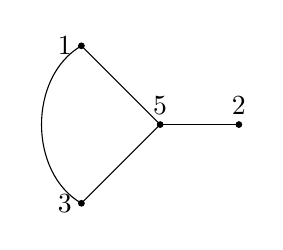
\begin{tikzpicture}
                        \filldraw (0,0) circle (1pt) node[left] {3};
                        \filldraw (0,2) circle (1pt) node[left] {1};
                        \filldraw (1,1) circle (1pt) node[above] {5};
                        \filldraw (2,1) circle (1pt) node[above] {2};
                        \draw (0,0) -- (1,1) -- (0,2);
                        \draw (0,2) to[bend right=60] (0,0);
                        \draw (1,1) -- (2,1);
                    \end{tikzpicture}  \tab 
                    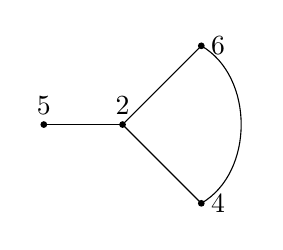
\begin{tikzpicture}                    
                        \filldraw (-1,1) circle (1pt) node[above] {5};
                        \filldraw (0,1) circle (1pt) node[above] {2};
                        \filldraw (1,0) circle (1pt) node[right] {4};
                        \filldraw (1,2) circle (1pt) node[right] {6};

                        \draw (1,2) -- (0,1) -- (1,0);
                        \draw (1,0) to[bend right=60] (1,2);
                        \draw (0,1) -- (-1,1);
                    \end{tikzpicture}
                
                    $\{1,3\} \to \{b, a\}$ \tab
                    $\{1,5\} \to \{b, c\}$ \tab
                    $\{2,4\} \to \{d, e\}$ \\
                    $\{2,5\} \to \{d, c\}$ \tab
                    $\{2,6\} \to \{d, f\}$ \tab
                    $\{3,5\} \to \{a, c\}$ \\
                    $\{4,6\} \to \{e, f\}$
                }{}
        \end{itemize}
        
    %\item   
        %\begin{itemize}
            %\item[a.]   Finish the adjacency matrix:
            
                %\begin{tabular}{c | c | c | c | c | c}
                    %& a & b & c & d & e
                    %\\ \hline
                    %a
                        %& \solution{0}{}
                        %& \solution{1}{}
                        %& \solution{0}{}
                        %& \solution{0}{}
                        %& \solution{1}{}
                    %\\ \hline
                    %b
                        %& \solution{1}{}
                        %& \solution{0}{}
                        %& \solution{1}{}
                        %& \solution{0}{}
                        %& \solution{0}{}
                    %\\ \hline
                    %c
                        %& \solution{0}{}
                        %& \solution{1}{}
                        %& \solution{0}{}
                        %& \solution{1}{}
                        %& \solution{1}{}
                    %\\ \hline
                    %d
                        %& \solution{0}{}
                        %& \solution{0}{}
                        %& \solution{1}{}
                        %& \solution{0}{}
                        %& \solution{1}{}
                    %\\ \hline
                    %e
                        %& \solution{1}{}
                        %& \solution{0}{}
                        %& \solution{1}{}
                        %& \solution{1}{}
                        %& \solution{0}{}
                %\end{tabular}
            %~\\~\\
            %\item[b.]   Fill out the degrees of each:
            
                %\begin{tabular}{ p{1cm} |p{1cm} |p{1cm} |p{1cm} |p{1cm} }
                    %a & b & c & d & e
                    %\\ \hline
                      %\solution{ 2 }{} % a
                    %&   \solution{ 2 }{} % b
                    %&   \solution{ 3 }{} % c 
                    %&   \solution{ 2 }{} % d
                    %&   \solution{ 3 }{} % e
                    %\\
                    %& & & & \\
                %\end{tabular}
        %\end{itemize}
        
        \hrulefill
        
    \item   
        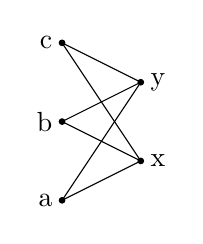
\begin{tikzpicture}
            \filldraw (0,0) circle (1pt) node[left]         {a};
            \filldraw (0,1) circle (1pt) node[left]         {b};
            \filldraw (0,2) circle (1pt) node[left]         {c};
            \filldraw (1,0.5) circle (1pt) node[right]         {x};
            \filldraw (1,1.5) circle (1pt) node[right]         {y};
            \draw (0,0) -- (1,0.5) -- (0,1) -- (1,1.5) -- (0,2) -- (1,0.5);
            \draw (0,0) -- (1,1.5);
        \end{tikzpicture}
        \solution{
            Example:
            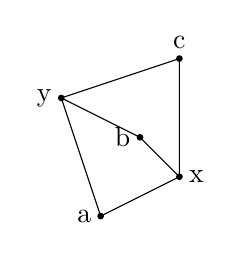
\begin{tikzpicture}
                \filldraw (0,0) circle (1pt) node[left]         {a};
                \filldraw (0.5,1) circle (1pt) node[left]         {b};
                \filldraw (1,2) circle (1pt) node[above]         {c};
                \filldraw (1,0.5) circle (1pt) node[right]         {x};
                \filldraw (-0.5,1.5) circle (1pt) node[left]         {y};
                \draw (0,0) -- (1,0.5) -- (0.5,1) -- (-0.5,1.5) -- (1,2) -- (1,0.5);
                \draw (0,0) -- (-0.5,1.5);
            \end{tikzpicture}
        }{}

        \newpage      
        
    \item   
        \begin{itemize}
            \item[a.]
                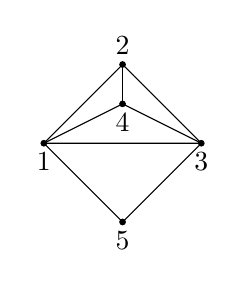
\begin{tikzpicture}
                    \filldraw (0,0) circle (1pt) node[below]{5};
                    \filldraw (-1,1) circle (1pt) node[below]{1};
                    \filldraw (1,1) circle (1pt) node[below]{3};
                    \filldraw (0,1.5) circle (1pt) node[below]{4};
                    \filldraw (0, 2) circle (1pt) node[above]{2};

                    \draw (-1,1) -- (1,1) -- (0,0) -- (-1,1);
                    \draw (-1,1) -- (0,1.5) -- (1,1);
                    \draw (-1,1) -- (0,2);
                    \draw (1,1) -- (0,2);
                    \draw (0,1.5) -- (0,2);
                \end{tikzpicture}

            \solution{
                1, 2, 4, 1 \tab 1, 3, 5, 1 \tab 2, 3, 4, 2 \\
                1, 3, 4, 1 \tab 1, 2, 3, 5, 1 (unbounded).
            }{}
            ~\\~\\
            \item[b.]
                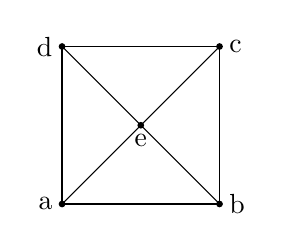
\begin{tikzpicture}
                    \filldraw (0,0) circle (1pt) node[left]{a};
                    \filldraw (2,0) circle (1pt) node[right]{b};
                    \filldraw (2,2) circle (1pt) node[right]{c};
                    \filldraw (0,2) circle (1pt) node[left]{d};
                    \filldraw (1,1) circle (1pt) node[below]{e};

                    \draw (0,0) -- (2,0) -- (2,2) -- (0,2) -- (0,0);
                    \draw (0,0) -- (1,1) -- (0,2);
                    \draw (2,0) -- (1,1) -- (2,2);
                \end{tikzpicture}

                \solution{
                    a, b, e, a  \tab    a, e, d, a  \tab d, e, c, d \tab b, c, e, b
                    \\
                    a, b, c, d, a (unbounded)
                }{}
        \end{itemize}
\end{enumerate}


\input{BASE-FOOT}
